\documentclass{article}

\usepackage{hyperref}
\usepackage{listings}
\usepackage{xcolor}
\usepackage{graphicx}
\usepackage{subcaption}
\usepackage{placeins}
\usepackage{pdfpages}

\graphicspath{{"pictures"}}

\lstset{
    basicstyle=\ttfamily\small,
    breaklines=true,
    numbers=left,
    numberstyle=\tiny,
    frame=single,
    keywordstyle=\color{blue},
    commentstyle=\color{gray},
    stringstyle=\color{orange},
}
\lstdefinelanguage{yaml}{
    morekeywords={true,false,null,y,n},      % Add keywords here
    sensitive=false,                        % Case insensitive
    morecomment=[l]{\#},                    % Line comments start with #
    morestring=[b]",                        % Double-quoted strings
    morestring=[b]',                        % Single-quoted strings
}

\setlength{\parskip}{1em}

\title{Chemical and Inventory Management System \\ SoFab Inks \\ Team 3}
\date{November 29, 2024}
\author{Hilton Benson, Blake Hourigan, CJ Johnstone, Maggie Jackey}

\begin{document}  
\maketitle
\clearpage
\tableofcontents
\clearpage

\section{Introduction\slash Executive Summary} 
\subsection{Introducing SoFab Inks}
SoFab Inks is a chemical manufacturing startup that was spun-out from the University of Louisville, Conn Center for Renewable Energy 
Research with support from the US DoE. SoFab inks focuses on accelerating the commercialization of Perovskite Solar Cells 
through the development and manufacturing of functionalized inks that improve cell efficiency, reduce module cost, and enable scalable 
manufacturing. \cite{sofabinks}
\subsection{SoFab Inks Inventory Management Problem}
SoFab Inks is doing important work in the field of solar cell technology, helping to drive humanity towards a cleaner, more energy 
abundant future. The problem, however, is that the team currently faces issues with managing inventory. These challenges prevent SoFab's
talented team from working on the most important aspects of their work. These challenges include expending valuable energy on menial 
tasks like locating inventory, managing a growing number of shipments manually, scouring inventory entries found across several 
Google Sheets or handwritten labels to pinpoint important product information, and more. 

To aid SoFab in these challenges, this semester Team 3 was tasked with developing a more efficient method of managing inventory items. 
To accomplish this, the team employed various existing software solutions, including database software, CRUD\footnote{Database term
for Create, Read, Update, Delete.} user interface software, and solutions to containerize this software together into one package. The 
team also developed custom software to provide features not available in the existing software solutions. 


\section{System Description}
The following sections describe the specifications that were formulated as a result of communication between Team 3 and the SoFab Inks
team. 
\subsection{Needs Assessment\slash System Requirements}
Following assignment to this project, the team assembled and met virtually with the SoFab Inks team for brief self-introductions, 
an overview of the current issues facing SoFab, and to gain an initial insight of what the SoFab team was looking for in a
solution to these issues. 

The SoFab team described the current state of inventory management at the company which included problems such as shipments arriving 
to incorrect customers, an inability to pinpoint important information about products as they progressed through the manufacturing 
process, and difficult to track remaining volumes of chemical products. In these discussions, SoFab also emphasized the importance 
of a solution begin \textit{simple and easy-to-use}. As the team is primarily constructed of chemical engineers or business people, 
technology was not a strength. 

The company also made it clear that the ability to generate item labels for internal tracking of 
should be a priority. These labels would allow members of their team to easily scan a barcode to view the details of an item. Finally, 
it was also made clear that the company also desired the ability to generate shipment labels for their products as well. These labels 
would differ slightly from their internal tracking label counterparts with the inclusion of chemical hazard information. This information
would be included as a way to reduce harm for customers handling SoFab's chemicals upon receipt.

After this initial discussion, Team 3 began to brainstorm potential solutions to the problems presented. Immediately, 3 main 
pieces of software jumped out at the team as critical pieces to what would be the final product.

\begin{enumerate}
    \item \textbf{A Database System} - In order to move the company away from the usage of Google Sheets and toward a more efficient, 
        safe and redundant, user-friendly solution, Team 3 knew it would be necessary to select an existing database software solution.
        While the team was unsure of what specific solution would be chosen, it was sure that one of these solutions would be required.
    \item \textbf{A User-Friendly Database Interface} - While a database solution would be an incredible improvement on its own, it 
        would be useless to the SoFab team if there were not a simple and easy way to interact with the underlying data. Again, the team
        was unsure of what specific solution would be chosen, but a few requirements from discussions with SoFab were clear. 
        \begin{itemize}
            \item \textbf{Clean, Simple, Easy-to-Use} - As previously discussed, SoFab was clear that a simple and easy-to-use solution
                was of paramount importance for the day-to-day usage of the product. 
            \item \textbf{Free and Open-Source} - While this requirement was not mentioned in the initial discussions with SoFab, this 
                requirement jumped out as important to Team 3 because this would help to avoid incurring additional costs beyond the 
                development cost that SoFab had already paid. 
        \end{itemize}
    \item \textbf{Software to Generate Internal and Shipment Labels} - After discussing the need for barcode and label generation software,
        the team found that it would likely be necessary to build custom software to meet the needs of the client. The requirements were 
        quite specific, and would not be available in any existing commercial product. These requirements certainly would not be made 
        available in any \textit{free and open-source} software.
\end{enumerate}
\subsection{Initial System Specification}
\label{sec:init-sys-specs}
Following the identification of the 3 main categories of software that would comprise the solution to SoFab's inventory management 
problems, Team 3 dove into research of each individual component to identify optimal selections. 
\subsubsection{Selecting a Database}
Firstly, it was important for Team 3 to become familiar with existing solutions that were \textbf{free and open-source}. 
This required conducting research on computer-science related websites and forums, and more general forums like 
Reddit. While a site like Reddit may not always be the most reliable source of information, it could provide a general sense of what 
people feel about particular software and how easy it is work with. 

Many databases fulfilling the free and open-source requirement were identified, including: PostgreSQL, MySQL, MariaDB, and SQLite. As 
many options were available to select from, it was important to look beyond this requirement and investigate techinical specificaitions
of these solutions. During this time it was discovered that \textbf{PostgreSQL} had several technical benefits over more popular 
rivals. PostgreSQL boasts of being a fully \textbf{ACID} compliant database system. With features such as \textit{Write-Ahead Logging},
which writes transactions to a log file to avoid pushing a full table(s) every time a transaction is committed, \textit{Multi-version 
Concurrency Control} which the PostgreSQL documentation describes as 

\begin{quote}``This means that while querying a database each transaction 
sees a snapshot of data (a database version) as it was some time ago, regardless of the current state of the underlying data. 
This protects the transaction from viewing inconsistent data that could be caused by (other) concurrent transaction updates on the 
same data rows, providing transaction isolation for each database session.''\cite{postgresql-mvcc}
\end{quote} 

Furthermore, PostgreSQL utilizes its \textit{Write-Ahead Log} to implement \textit{Point-in-Time Recovery} without the need of 
complete backup. Additionally, since the Write-Ahead Log contains all transactions since the previous system backup, one can 
return to the exact state of \textbf{any} \textit{point in time} between the most recent backup version and the current version. 
Team 3 felt that these benefits would be incredibly beneficial for SoFab's new database, which would be the central hub containing 
the whereabouts and remaining inventory of their lab. This database would also contain important product information which if lost 
or damaged could have severe consequences for their business. 

Beyond technical considerations, ease of use was of great consideration when selecting a database, and luckily, PostgreSQL 
benefits from being very easy-to-use. PostgreSQL has an additional software called \textbf{PgAdmin4}, a project led by a core developer of 
PostgreSQL! This software integrates very well with PSQL\footnote{PSQL is short for PostgreSQL.}
This software provides a GUI that allows developers to interact with the database, run queries, add and edit tables, view ERDs
\footnote{ERD stands for entity relationship diagrams.} for tables, and much more. This would simplify team members development tasks
significantly and enable faster production. 

For the reasons stated above, PostgreSQL was selected as the database software of choice for this project. 
\subsubsection{Selecting an Interface}
While PostgreSQL would be a great choice to build a database for SoFab inks, this software alone - as stated previously - would be 
useless to the SoFab team by itself. Team 3 needed to produce a user interface that was simple, user-friendly, and would be capable 
of fulfilling all of SoFab's functional requirements. Team 3 scoured the internet, searching for a solution that would fulfil these 
requirements. Eventually, the open-source software Budibase was found. Upon investigation into Budibase, it was discovered that this 
software could be self-hosted, and if self-hosted, was \textit{free-to-use}. This immediately fulfilled two requirements, so the team
installed the software locally and began to interact with it to determine if it could fill the user-friendliness and functional 
requirements discussed previously. 

It was found that Budibase functions in a manner similar to that of website builders like ``Wix'' or ``Squarespace''. An architect
has the ability to connect to an existing database, 
then can select from existing templates based on the type of project at hand, and even use templates for types of pages to use. The 
architect can select between form-type templates where the user can edit or insert information about a row in a database table, or table-type 
templates where the user can view large amounts of data at a glance. 

Additionally, one can drag and drop pre-made components from the sidebar, and arrange them as they see fit. These components can 
connect to any data source in the database. Data sources include standard database tables and even custom queries to provide maximum 
customizability. 

While using a builder software like Budibase reduces the complexity in creating CRUD apps, they can pose a challenge in that all 
documentation and 
instructions for using the software provided strictly by Budibase themselves. The self-hosted Budibase community is not 
very large, so if an issue arises, an architect may be left to themselves to resolve it if that issue is not covered
in the existing documentation. 

Thankfully, however, the Budibase team has prioritized documentation, with instructions on how to use their many available 
components in various ways. They have created a page dedicated to the use of their platform, self-hosting instructions and guidance, 
component use, connecting the service to the database software in use, and much more. \cite{budibase-docs} The team also provides 
many instructional videos and how-tos on their website and on their company YouTube page. \cite{budibase-youtube}

\subsubsection{A Language for Custom Software}
After selections were made for database and user-interface software, discussions were held on the topic of how the final major piece 
of the software stack - the custom label printing interface - would be constructed. Team 3 understood SoFab's requirement for this 
deliverable - that the software create printable labels to place on their inventory - but Team 3 imposed additional requirements
that would support the team to fulfill the company's requirement. These requirements were identified as follows. 
\begin{enumerate}
    \item \textbf{Familiarity} - The most important requirement that was identified by Team 3 during these discussions was familiarity 
        among team members with various programming languages. Due to semester imposed time constraints, it would be important to hit 
        the ground running, without additional challenges of learning an unfamiliar programming language. A consensus was reached that 
        team members all had prior experience with \textit{Python}. This prior experience, paired with the languages intuitive syntax
        made Python an attractive choice with regard to this requirement. 
    \item \textbf{Community Support\slash Libraries} - Another important requirement concerning the selection of an optimal programming 
        language to develop this new software was community support and library availability. Once again, \textit{Python} was identified
        as a language with great strength in this aspect. Python is known for its extensive library support, with over 589,000 projects
        in the `pypi' Python package repositories. \cite{pypi} Packages were identified that would allow Team 3 to easily generate 
        barcodes, generate PDF outputs, and read from PostgreSQL databases. These features attributed to the appeal of Python for the 
        development of this deliverable. 
    \item \textbf{Reliability\slash Durability} - The two requirements previously discussed were found to be great strengths of the 
        Python language. However, an additional consideration for selection for this custom software was the durability of the language. 
        A reasonable argument could be made that the responsibility of ensuring reliability and durability of code lies with the 
        programmer, and not the language that a programmer may employ. However, humans have proven to be much less reliable than 
        machines in many domains with defined rules. 

        Recent developments in the programming domain such as the Rust language have built 
        this fact of reality into the fabric of the language. These such languages provide memory safety by default, meaning that the 
        programmer must have advanced knowledge of the language before performing potentially dangerous programmatic actions. Rust also 
        provides an excellent ecosystem of tools such as `Cargo' which both manages project dependencies and provides an easy method to
        run and test written code. Rust offers many benefits that Team 3 believed could be incredibly beneficial for a project that would 
        need to be consistent and reliable day-to-day at SoFab Inks.
    \item \textbf{Speed\slash Efficiency} - A final major consideration in choosing a programming language was the speed that the chosen
        language would provide after development. Performance is \textit{always} an important consideration, but this was  
        especially true with Team 3's plan to install many pieces of software on one machine on final deployment. On this point, Rust 
        again was found to have great advantages. Compared to Python, Rust is far more efficient, as it is 
        a compiled language. This means that at program run-time, no `interpretation' of the code is required. This essentially shifts much
        of the heavy computational lifting to the code `compilation' process, allowing the program to execute more efficiently at run-time. 
\end{enumerate}

Upon reviewing the major points of consideration, Team 3 decided that Familiarity and Comunity Support\slash Library availability were 
critical attributes in the lanuage selection process. While a language such as Rust provided significany boosts in execution time
and Reliability, both of which would be beneficial to the end user, it was decided that the team had too little familiarity with this 
language. Learning a new language as a team would increase the complexity of the project too greatly, and endanger Team 3's ability to
produce a satisfactory product on-time. It was for these reasons that Team 3 decided to select Python as the language of choice for the 
development of this additional software, pending approval by the SoFab team during the next meeting. 


(External design document) 
    EAC 1. Identify, formulate, and solve complex engineering problems by 
    applying principles of engineering, science, and mathematics and CAC 1. 
    Analyze a complex computing problem and to apply principles of computing 
    and other relevant disciplines to identify solutions) 

\subsection{Final Specifications}
Little changed with regard to the major required specifications of chosen software over the course of this project. While minor changes
were implemented in requirements with regard to specific data tracking points or tracking methods, these could all be accomodated within
the existing framework. For this reason the majority of the final technical specifications were set during the meeting that followed
Team 3's discussion of initial specifications for the system.

Team 3 met with the SoFab team to discuss the specifications that Team 3 had arrived at as results of the prior discussions. The team 
wanted to ensure that these specifications aligned with the needs and vision of the company. Team 3 proposed the previously discussed
database and user-interface solutions, with brief technical demonstrations showcasing the potential of these pieces of software as 
solutions to the inventory management problem. SoFab responded positively, with few notes with regard to the technical decisions reached 
by Team 3. 

For these reasons the following selections were made final as software solutions for this project.

\begin{itemize}
    \item \textbf{Database System} - PostgreSQL
    \item \textbf{User-Interface\slash CRUD Frontend} - Budibase
    \item \textbf{Programming Language for Custom Software} - Python
\end{itemize}
\subsection{System Diagrams} 
Once specifications were made, it was important to visualize processes for each system.  

Through diagrams, Team 3 was able to define key components and interactions prior to implementation.  The systemm, shown in 
Figure \ref{fig:sys_diagram} consists of three main components: the Frontend, Middleware, and Backend (Database). 

\begin{enumerate} 
    \item \textbf{Frontend (Budibase)} - The user interacts with a web-based interface, with options to create, remove, and edit.  
    This interface allows users to request data, view reports, and generate PDFs.  
    \item \textbf{Python Program} - The Python program allows for interactions with the PostgreSQL database; 
    allowing users to fetch or manipulate data, and generates PDF label documents based on the data.  
    \item \textbf{Backend (PostgreSQL)} - The PostgreSQL database represents the data storage layer, containing all data for 
        the system.  
    It's referenced across all system components, whether for display in Budibase or for generating label PDFs on the python program. 

     \begin{figure}[h]
        \centering 
        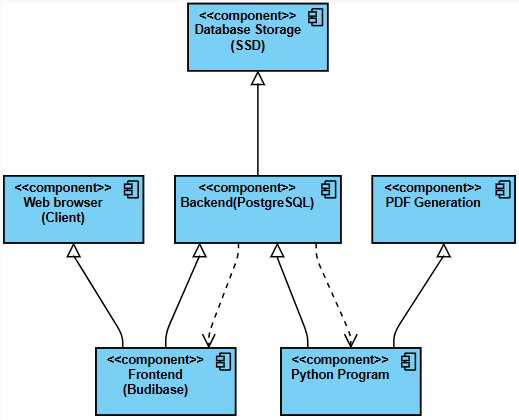
\includegraphics[width=0.5\linewidth]{pictures/sys_diagram2.png} 
        \caption{Overview of frontend, backend, and middleware interactions.} 
        \label{fig:sys_diagram} 
    \end{figure} 
        \FloatBarrier
\end{enumerate} 
\subsection{Hardware Overview Diagram} 
Hardware architecture \ref{fig:hardware} includes a desktop hosting the PostgreSQL database, which serves as the central data 
repository. To access this repository, web-based interface \textit{pgAdmin} in addition to vpn-service \textit{Tailscale} where 
remote connections were established. Both of these methods allowing team members to connect from their laptops securely and 
manage the database from different locations. 

\begin{figure}[h]
    \centering 
    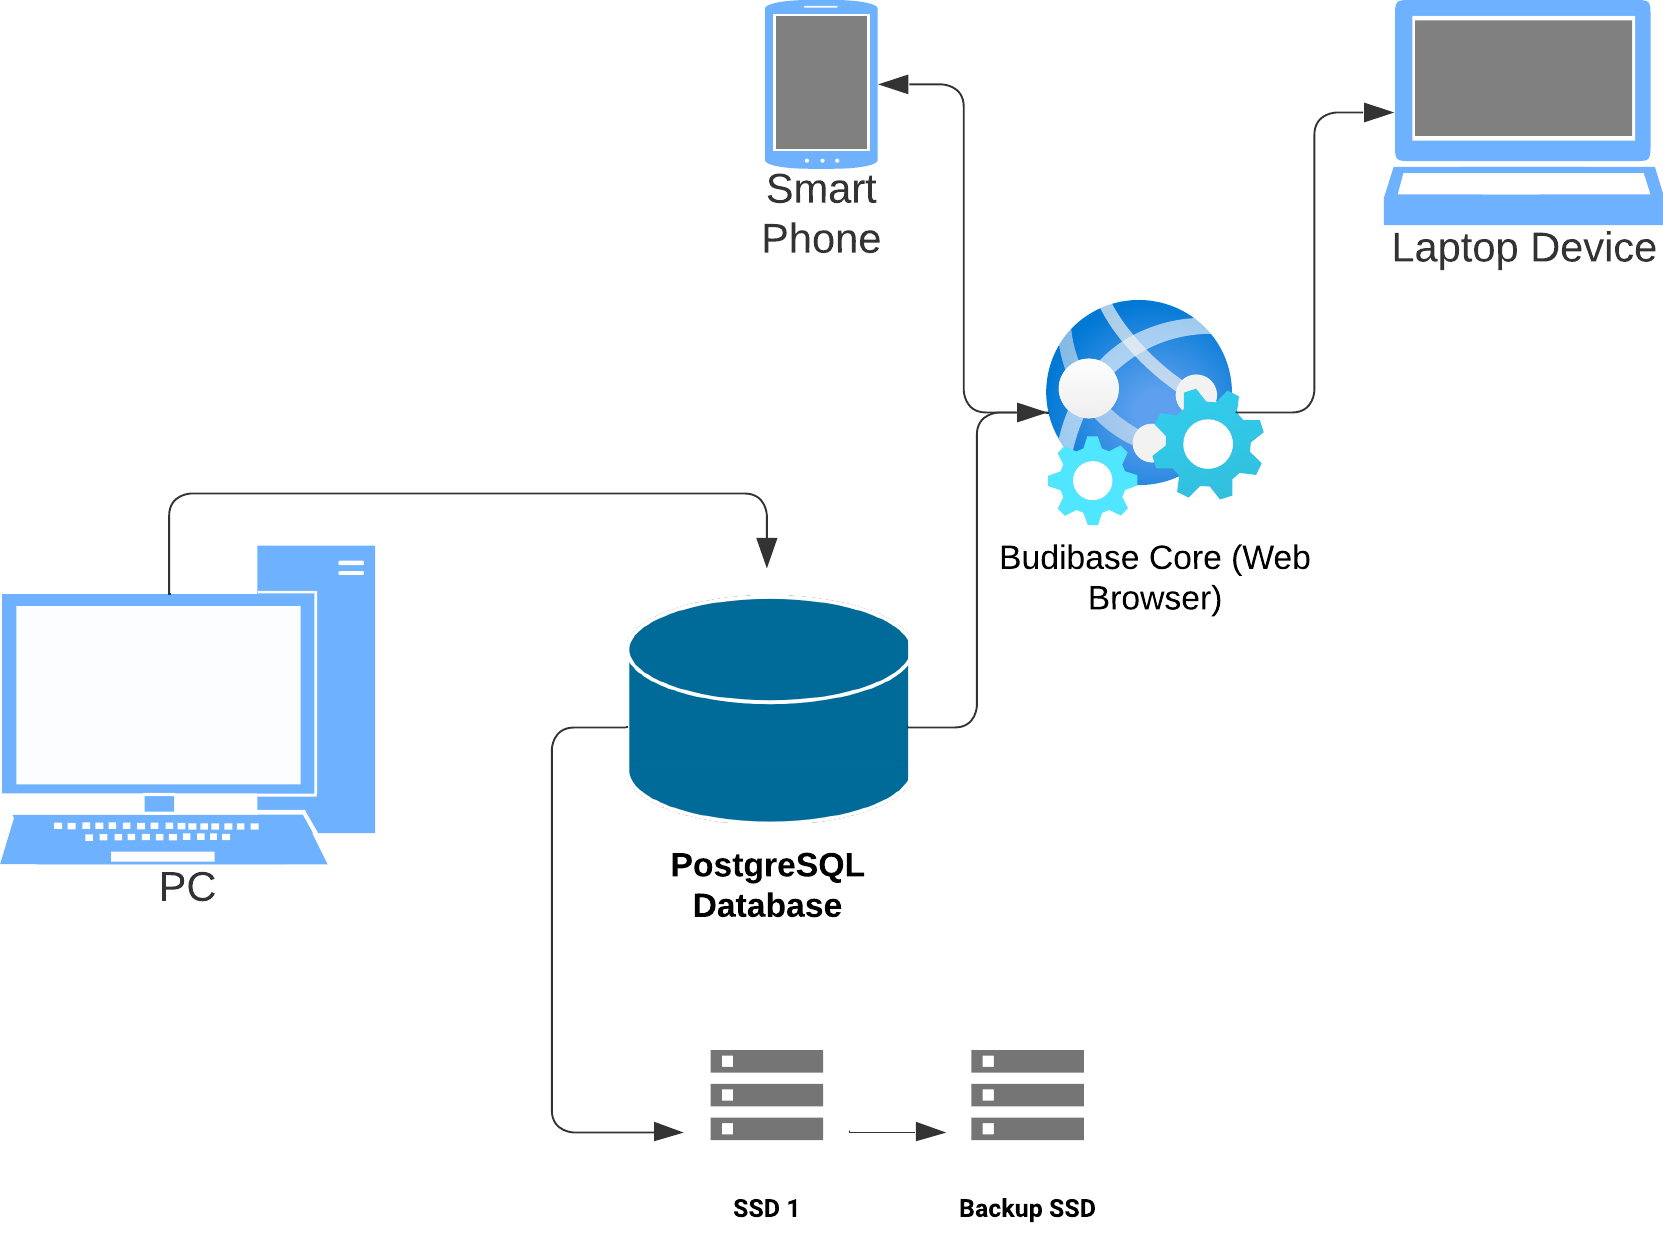
\includegraphics[width=1\linewidth]{pictures/hardware_diagram.png} 
    \caption{Hardware components and their connections} 
    \label{fig:hardware} 
\end{figure} 
\FloatBarrier

\subsection{Software Overview Diagram} 
A diagram was needed to show interactions between software. Budibase and the custom Python application both integrate with pgAdmin,  
which serves as the interface for managing the PostgreSQL database.  
\begin{enumerate} 
    \item \textbf{PostgreSQL Database Integration} -  
    The following diagram \ref{fig:database_diagram} represents early design stages of the PostgreSQL database.  
    The diagram focuses on the key tables involved in the company’s batch process,  
    representing a streamlined version of the entire database architecture. 
    The core table for the batch process is ‘Batch Inventory’, which holds fields such as 
        \textit{ID} (which is used as a unique identifier across all tables),  
    hazard information, and other critical fields. 

    \begin{figure}[h!] 
        \centering 
        \begin{subfigure}[b]{\textwidth} 
        \centering 
        \includegraphics[width=7cm]{"database_sys_diagram.png"} 
        \caption{Batch Process Info Tracking Tables} 
        \label{fig:database_diagram} 
        \end{subfigure} 
    \end{figure} 
        \FloatBarrier

    \item \textbf{User Interface for Database Interaction  \textit{(Budibase)}} - First step involves user login to the web interface 
    On successful login, the user is directed to the Home Screen, allowing for product search through ID.  
    Based on the Product ID entered, the system will determine the next screen based on the product's type in the inventory database.  
    The product type directs the flow to  
    \textit{General Inventory}, \textit{Chemical Inventory}, or \textit{Product Inventory}. 
    Additional screens include order, customers, and analytics. The following diagram \ref{fig:bb_software_diagram}  
    visualizes this process 
        \begin{figure}[h]
        \centering 
        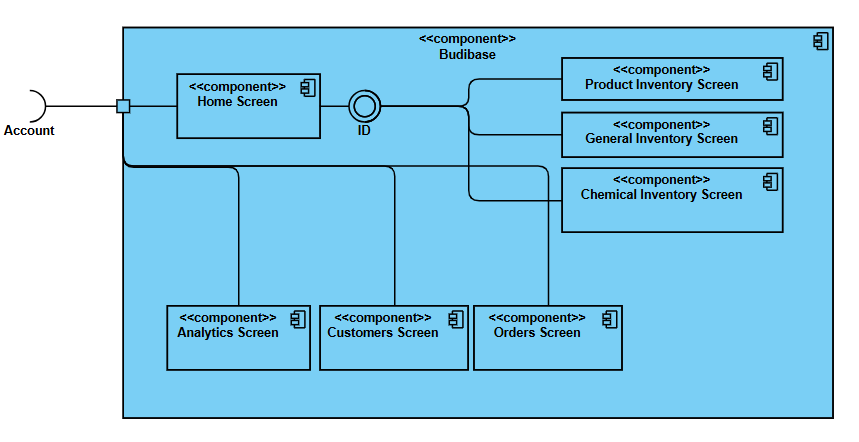
\includegraphics[width=0.5\linewidth]{pictures/bb_diagram2.png} 
            \caption{Structure of web interface (\textit{Budibase})} 
        \label{fig:bb_software_diagram} 
    \end{figure} 
    \FloatBarrier

    \item \textbf{Python Application for \textit{Chemical Data Entry}} - The flow begins with the user launching the program, which 
        prompts them to choose from one of three inventory types. After selecting the appropriate type, the user enters the 
        relevant chemical information. The application then generates a unique product ID for the item and, finally, adds the 
        entered data to the database for storage and future reference. Each step in the process is clearly mapped to ensure 
        efficient data handling and accurate inventory management (Figure \ref{fig:appsysdiagram}).  

    \begin{figure}[h!] 
         \centering 
         \includegraphics[width=10cm]{"python_app_sys.png"} 
         \caption{Adding user entries to inventory tables in PSQL} 
         \label{fig:appsysdiagram} 
     \end{figure} 
\end{enumerate} 

\subsection{Economical, Technical, and Time Constraints}
Over the course of this project, several constraints were imposed and revealed to Team 3 that limited the available tools for this 
project. These constraints fell under three main categories, each of which will be discussed in its respective section below. 
\subsubsection{Economic Constraints}
Firstly, Team 3 experienced economic constraints, financially limiting software solutions available as tools for this project. Team 3 
was limited economically primarily due to the identified requirement that utilized software be \textit{free and open-source}. As 
discussed previously, this requirement was identified to avoid incurring subscription costs charged to SoFab following development of 
the project solution. This limitation significantly limited the software tools available to Team 3 for development. 

Additionally, Team 3 was constrained economically due to the inability to provide development hardware to the SoFab team upon project
completion. Unbeknownst to Team 3 early in the semester, hardware that was purchased to facilitate development of the project would be 
unable to be transferred to the on-site location upon completion. Luckily, the university approved the request to transfer necessary 
hard drives containing critical database information upon project completion, but did not approve this request for other hardware 
necessary for this projects successful completion, such as a barcode scanner or label printer. For this reason the team was economically 
constrained and encouraged to develop a solution to SoFab's inventory management problem on the smallest budget the team could manage. 

Similarly to the previous constraint, meeting this constraint would be important to ensure that SoFab would incur the smallest possible
cost upon project completion. Team 3 wanted to deliver a project that contained as much of the desired functionality as possible, while
avoiding extra purchases like barcode scanners or product label printers. 

The team will expand on the specific solutions implemented to meet project requirements in the face of these constraints, however, the 
main ways in which economic constraints were addressed follow below. 

\begin{enumerate}
    \item Free and Open-Source Software
    \item Software Implementation of Hardware Features\slash Creative Use of Existing Hardware
\end{enumerate}

\subsubsection{Technical Constraints}
The next primary factor which constrained Team 3 during the development of the solution their technical ability and technological 
constraints. The limitations in technical ability discussed here coincide with time constrains, however technical ability specifically 
will be discussed in this section. As discussed in Section \ref{sec:init-sys-specs}, Team 3 was limited technically in that all team 
members had the most familiarity with one programming language - \textit{Python}. This imposed several technical limitations including 
reliability and efficiency that were traded for familiarity, ease-of-use, and library availability. The Rust programming language's 
memory safety features, combined with its status as a compiled language held much in the way of potential benefits for the development 
of this project. However, due to Team 3's unfamiliarity with the language, these potential benefits became limitations by use of Python, 
which faces challenges both with reliability and efficiency. 

Additionally, Team 3 was consrained technologically by installation hardware. Upon completion, this project's software stack would 
be installed onto SoFab's main laboratory computer. This software stack would act as a server on the local area network to field requests
from mobile devices for ease-of-use and convenience. It was for this reason that Team 3 was obligated to be mindful of resource usage 
regarding installed software, and aware of the computational cost of adding further software. The installation site would be used for 
other tasks besides this inventory management system, and therefore the system needed to function efficiently to avoid slowing down 
other operations and tasks conducted on the lab computer. 

Specific action taken to avoid concerns regarding these constraints is discussed in Section \ref{sec:det-imp}, however a general outline
is provided here. 
\begin{enumerate}
    \item Mindfulness Regarding Existing Lab Hardware
    \item Implementing Only Critical Software Solutions
    \item Writing Efficient Python Code
\end{enumerate}
\subsubsection{Time Constraints}
The main factor which imposed constraints on Team 3 during the Fall 2024 semester was time. The team had approximately 3 months to develop
a solution that would satisfy the requirement of the SoFab team, and this meant that Team 3 needed to act fast to develop their product.
This deadline itself imposed constraints on the team, such as how often and with what intensity the team needed to act, however it was 
also the primary factor in imposing technical limitation. Team 3 simply had no time to learn a new programming language 
comprehensively 
prior to implementing a solution. This was the driving factor in the selection of a familiar and well-supported programming language 
such as \textit{Python.} 

Furthermore, meeting dates with the SoFab team imposed constraints in that signicant progress was expected of the team approximately
every 2 weeks, when meetings would occur. After one of these meetings had concluded, the team had 2 weeks to implement early versions
of the discussed features to be showcased at the next meeting. This imposed an intensity that Team 3 needed to work with to be prepared
for every meeting. 

\section{Detailed Implementation} 
\label{sec:det-imp}
The below sections include the specific actions and steps taken by Team 3 to develop the solution to SoFab Inks inventory management
problem with project requirements and constraints accounted for. 
\subsection{Hardware Detailed Implementation}
While the solution developed over the course of this project was constructed primarily of software components, some hardware components 
were required to meet and exceed the requirements of SoFab Inks. The primary hardware components are covered in detail below.
\subsubsection{A Home for A Database}
\label{sec:server}
As discussed in previous sections, in order to develop software that improved significantly on SoFab team members experience of managing
inventory, a database system was required. Once this was decided, the main point of emphasis was how to implement this requirement as 
safely as possible. Team 3 wanted to ensure with certainty that SoFabs sensitive and irreplaceable company data would be both secure 
and redundant to a avoid a catastrophic data loss scenario. This requirement however was not without mild cost. 

The security of the database was primarily a matter for the software implementation, however, redundancy required multiple storage locations
to ensure multiple independent copies of the database are available at any given time. For this reason Team 3 decided to purchase two 
1 terabyte solid-state storage drives, intended to each contain separate copies of the database. One of these disks would contain the 
current working version of the database at all times, while the other drive would contain backups that would be conducted on a daily 
basis. The team could even write a script in such a way to keep record of each backup instead of overwriting the backup each day with the 
new copy. This would allow the team to inspect the database at any given point in its history if required. 

Furthermore, investing in these drives at the beginning of the project life-cycle improved the experience of the transition to the 
installation site significantly. Because the team was able to develop the project on the purchased SSDs,\footnote{SSD is a computational
term for Solid State storage Disk.} when the project was transferred on-site, the team could simply bring the drive containing the up-to-date
software stack, point the lab computer to this disk, and have the project up-and-running. 
\subsubsection{A Barcode Scanning Interface} 
An additional piece of hardware needed to meet the full requirements of the SoFab team was a barcode\slash QR code label scanner that 
would allow the team to simply scan product to view their corresponding inventory details. While the SoFab team would be unable to keep 
the scanner that Team 3 purchased for development due to university rules, this product was inexpensive and in SoFab Inks' reasonble price
range. The team conducted research into barcode scanning technology to discover what attributes made a good scanner. 

Team 3 found that most barcode capable hardware scanners could double as QR code scanners, with little differences in feature sets between
available models. For this reason the team sought an affordable wireless model that would allow SoFab to walk around their laboratory and 
scan products instead of being required to retrieve products first. The implementation of this barcode scanning technology required little
beyond purchasing the product. Once received, Team 3 could simply plug the scanner's bundled USB dongle into any computer, scan a barcode 
or QR code while inside a text field, and the scanner would take care of the rest. This purchase made the development of this 
feature simple and instantly partially fulfilled a requirement set out by SoFab Inks for their inventory management system. 
\subsection{Software Detailed Implementation}
The vast majority of effort expended by members of Team 3 this semester was in the domain of software. The team worked to utilize a 
combination of existing and custom-built software to provide an inventory management system that would satisfy requirements laid out 
by SoFab Inks. The individual pieces of software that played major roles in constructing this solution are discussed at length in the 
below sections.
\subsubsection{A Home Development Server}
Due to the nature of the software being developed, Team 3 identified a need to create a centralized server that would allow members to 
access the software from any location at any time. During the early weeks of development, the team was using existing tools and 
services to develop a solution such as PostgreSQL and Budibase instead of writing custom code. Development with these services would 
benefit substantially from running on a centralized server that could be modified by any team member. This would be far more efficient 
than developing solutions individually and compiling them into one solution at a later time. 

An added benefit of creating a centralized server where all development would take place was that this server would closely mimic the 
conditions of final installation. Upon installation, the software stack would be deployed on a single computer that would serve all 
clients on a local area network. This experience would allow the members of Team 3 to work with an experience closer to that of an end 
user. This allowed team members to experience bugs that would appear at the installation site and fix them as they arose. 

To construct a home server that would host all services required for this project and allow all Team 3 members access, a computer 
was set-up at a members home and given a static IP. This static IP would allow DNS services and the home router to find a constant path 
to the services to be accessed. Next, it was time to install all the existing services that would be required to develop the project. This 
software will be discussed at length in Section \ref{sec:docker}. All services were installed and initialized. 

Next, a Nginx server 
running on another computer was configured as a reverse-proxy. A reverse-proxy is a service that acts as an intermediary for servers or 
services running on a local network. A reverse proxy intakes network requests and forwards them to the server where they are hosted. 
The benefits that a reverse-proxy offers to users is that only one 
port is required to be exposed to the internet. This reduces the number of open ports on a network, offering security benefits. Additionally,
reverse-proxies can be configured to use HTTPS,\footnote{Hypertext Transfer Protocol \textit{Secure.}} also enhancing the security of data 
\textit{transmission}. Finally, reverse-proxies can also provide load balancing services, reducing strain on any one server on the 
network. 

\subsubsection{Docker-Compose}
\label{sec:docker}
Docker - and its supplemental software Docker-Compose and Docker Desktop - played a pivotal role during the development of this project.
Docker is a software that allows applications to be packed into `containers'. This allows these pieces of software to run in isolation from 
other software, be more easily configured, and be isolated from the host system network which can enhance software security. While Docker 
containers share similarities with classical virtual machines in that they provide environments that are isolated from the host machine, 
Docker containers differ in a few major respects that are important to note in this context. 

Virtual machines are known for the performance penalty that accompanies their use. This is because virtual machines are tasked with 
emulating an entire operating system, which is a very complicated and resource intensive task. Docker containers work to alleviate 
this performance problem by \textit{sharing the host's operating system kernel}. This allows Docker to focus on the application 
software itself, without the need to emulate existing operating system features. 

Expanding on these benefits, Docker-Compose provides the ability to roll multiple Docker containers into one centralized script, 
where all software to be used for a given project can be managed at once. One can specify version numbers, customize network configurations,
assign storage mounts,\footnote{Storage mounts are locations in a computer where files are located.}, allocate extra resources,
\footnote{An example of an extra resource would be allocating GPU resources for a container.} and more. 

The incredible benefits that 
this provides when developing an application to be deployed on another system cannot be overstated. What Docker-Compose allowed Team 3 
to do over the course of this project is to develop a software stack with versions of software that were compatible with one another. The
team installed this software on a Windows 11 machine to mimic the operating system in use at the site of eventual installation, reducing 
possible complications with system migration. Using these methods, Team 3 could be confident when the time for system 
migration came, that all software would be compatible and work together smoothly, keeping all existing data intact. 

This technology removed a great burden from Team 3, and the effort placed into creating a stable software stack through Docker-Compose 
was rewarded upon migration to SoFab's laboratory in late November 2024. This will be explained in greater detail in a later section.
The software that was integrated into this Docker-Compose stack included the database software PostgreSQL, the database management 
software PgAdmin4, and database frontend design software Budibase. 

Most developers that provide the ability to deploy an application via Docker provide example Docker-Compose scripts defining the 
critical application configurations and environment variables to deploy the application. This was very beneficial to Team 3 for the 
development of this software stack, as examples for deploying PostgreSQL, PgAdmin4, and Budibase were found, accelerating deployment.
\cite{dockerhub-postgres} \cite{dockerhub-pgadmin} \cite{budibase-docker-compose}A sample of the final Docker-Compose Script is 
included below. 

\begin{lstlisting}[language=yaml]
 postgres:
   image: postgres:16
   volumes:
     - type: bind
       source: "D:/Docker Data/postgres_data"
       target: /var/lib/postgresql/data
   ports:
     - "5432:5432"
   restart: always
   container_name: postgres
   # set shared memory limit when using docker-compose
   shm_size: 128mb
   # or set shared memory limit when deploy via swarm stack
   environment:
     POSTGRES_PASSWORD: {POSTGRES_PASSWORD}
   extra_hosts:
     - "--add-host host.docker.internal:host-gateway"

 pgadmin4:
       image: elestio/pgadmin
       restart: always
       environment:
         PGADMIN_DEFAULT_EMAIL: ${ADMIN_EMAIL}
         PGADMIN_DEFAULT_PASSWORD: ${ADMIN_PASSWORD}
         PGADMIN_LISTEN_PORT: 8080
       ports:
         - "0.0.0.0:8080:8080"
       volumes:
         - pg_admin_data:/var/lib/pgadmin

volumes: 
  pg_admin_data:
\end{lstlisting}
\subsubsection{PostgreSQL}
Once the Docker-Compose script was defined and all software was deployed on the home server machine and exposed to all Team 3 members, 
application specific configuration began for PostgreSQL. User accounts were created (Figure \ref{fig:psql_users}) for each team member,
and credentials were distributed. Team 3 then initialized the database for the project (Figure \ref{fig:psql_dbs}), and set 
user privileges. PosgreSQL's user creation tool was utilized to add an additional account `database dev' which would be given privileges
to read, add, create, and delete on the database. These permissions could then be applied recursively to each user account, streamlining
the permissions process. 

\begin{figure}[h!]
    \centering
    \begin{subfigure}[b]{\textwidth}
        \centering
        \includegraphics[width=10cm]{"postgres_users.png"}
        \caption{Viewing existing users in the PSQL CLI interface.}
        \label{fig:psql_users}
    \end{subfigure}
    \begin{subfigure}[b]{\textwidth}
        \centering
        \includegraphics[width=10cm]{"postgres_dbs.png"}
        \caption{Viewing existing tables in the PSQL CLI interface.}
        \label{fig:psql_dbs}
    \end{subfigure}
    \caption{}
    \label{fig:posgres_cli}
\end{figure}
\FloatBarrier

\subsubsection{PgAdmin4}
With the database initialized, the team could begin work on constructing a relational database in PSQL\footnote{PSQL stands for PostgreSQL.}
that modeled the daily workflow in the SoFab Inks lab. However, Team 3 felt that it would be quite inefficient to develop in the 
PSQL CLI\footnote{CLI stands for Command Line Interface in a computer terminal.}. Members felt that it would be difficult to grasp the 
relations in a database and quickly view the attributes of a database with this interface. This would be especially true due to the 
length of time members
had gone without working on database systems. Unfamiliarity would lead to frustration and confusion through this method of interaction. 
For this reason members of the team began to seek out another way to interact with a database system with a graphical user interface. 

Quickly, members found that there existed a GUI\footnote{Graphical User Interface.} tool build specifically for PSQL called `PgAdmin4'. 
Best of all, this software was developed by a core member of the PSQL team! PgAdmin4 boasted features such as graphical management of 
existing attributes including database schemas, tables, types, trigger functions, and more. This would allow the team to manage the 
database visually in a way that would allow members to quickly and easily learn the tools available at their disposal in PSQL. Additionally,
this tool allowed for the execution of database queries, giving developers all the power of CLI PSQL in addition to the GUI tools. 

PgAdmin4 was deployed in the project's Docker-Compose script and deployed alongside PSQL. Once deployed, user accounts were created and 
configured to access the PSQL database under these accounts. At this stage Team 3 could begin constructing the database while avoiding
the overwhelming nature of a CLI tool to interface with the database system. Examples of the deployed instance after the insertion of 
tables can be found in Figures \ref{fig:pg_admin_tables}, and \ref{fig:pg_admin_queries}. More images can be found on PgAdmin4's webpage.
\cite{pgadmin-screenshots}

\begin{figure}[h!]
    \centering
    \begin{subfigure}[b]{.45\textwidth}
        \centering
        \includegraphics[width=6cm]{"pg_admin.png"}
        \caption{Viewing existing tables in PgAdmin interface.}
        \label{fig:pg_admin_tables}
    \end{subfigure}
    \begin{subfigure}[b]{.45\textwidth}
        \centering
        \includegraphics[width=6cm]{"pg_admin2.png"}
        \caption{Running PostgreSQL queries inside PgAdmin4.}
        \label{fig:pg_admin_queries}
    \end{subfigure}
    \caption{}
    \label{fig:pg_admin_figs}
\end{figure}
\FloatBarrier

In regard to the construction of the database, the same general process was followed for three primary forms of inventory in use 
at the SoFab team's lab. These consisted in `Product Inventory' which contained information about the company's products, 
`General Inventory' which contained general lab items such as beakers and shipping boxes, and `Chemical Inventory' which the 
company used as ingredients to their products. SoFab desired to have information about these items at each stage in their life-cycle. 
While this cycle changed depending on the type of inventory an item originated from, the process of creating tables to accomplish this
effect would remain the same. 

The general process follows below.
\begin{enumerate}
    \item \textbf{Create a Table for the \textit{Item}} - A table would be created for the type of inventory item, containing any 
        \textit{static}, or, constantly present, information about this type of item. This item would also contain the \textit{ID}, 
        which would be used to link each row, which represented one item, to related rows in other tables. 
    \item \textbf{Create a Table for Each Life \textit{Stage}} - Next, team members would construct tables that represented a stage in a 
        product's life. For example, the `Product' inventory may have a product table containing the ID of this product, chemicals used to 
        create this product, and in what amount, and other related information. Then, for each stage in a manufacturing process, 
        tables could be generated that would track specific information about actions performed on the item at this step. This was an
        important attribute, as this would give SoFab the ability to easily review the histories of successful batches, and be able to 
        recreate the product as closely as possible. 

        Similar steps would be followed for other categories of items, tracking information at every step related to an item that was 
        necessary as instructed by SoFab team members. 
    \item \textbf{Building Table \textit{Relationships}} - An important last step in the creation of the database is creating links 
        that connect tables together in terms of their relation to one another. This was generally accomplished by linked item IDs to 
        each other via `foreign keys', that helped the database understand the connections between different tables. A major benefit of 
        this relation creation is that it enables automatic generation of ERD\footnote{Entity Relationship Diagram.} diagrams. These 
        diagrams aid developers by visually representing database tables. An example of an ERD for this database can be found in 
        Figure \ref{fig:pg_admin_erd}.
\end{enumerate}

\begin{figure}[h!]
    \centering
    \includegraphics[width=12cm]{"pg_admin_erd.png"}
    \caption{ERDs help developers understand how tables are related.}
    \label{fig:pg_admin_erd}
\end{figure}
\FloatBarrier

\subsubsection{Budibase}
\paragraph{Why Budibase?}
At this stage of development, Team 3 had constructed a functional database system that could store all required information for SoFab 
Inks' inventory. However, the current interaction system of PgAdmin, while helpful to developers, would be incredibly cumbersome 
for an end user to use on a daily basis. The methods by which items would be displayed would be confusing and generally unhelpful. For 
these reasons, it was necessary to add another software solution to the existing stack to enable SoFab Inks to be able to intuitively 
view the database entries, and better understand their data. The interface, as stated previously, needed to be clean and easy-to-use, 
free and open-source, and the added touch of a visually appealing system would be appreciated. 

The team began their search into database systems with these constraints in mind. The requirement of a free and open-source system 
significantly reduced the available solutions for this deliverable, however one solution seemed to check all the required boxes. 
`Budibase' is a company that produces a database CRUD software that allows users to easily construct clean, simple, visually appealing
interface software. The company's software functions in a method that is similar to that of website builders `Wix' or `Squarespace'. 
The software can connect easily to many of the most popular database software solutions on the market, including PSQL. 
Users have the ability to choose from existing template pages as a starting point and, from there, drag and drop any one of the many 
available data components into existing pages. These components can connect to any data source existing inside of the connected database
including tables and, more importantly, queries. Queries allow users to construct custom tables that fit certain criterion in a database,
and act as a kind of filter to find only data that contains specific values. 

These technical specifications excited Team 3 as they would allow the development of an intuitive system and would provide a 
straightforward development experience. However, the most important requirement of the selected software were the cost of continued use
and the open or closed source nature of the project. Luckily, Budibase offers a self-hosted plan which allows users to run the software 
on a local machine with up to 5 administrative accounts and up to 20 user account completely free-of-charge. Budibase is also open-source,
and has a rich documentation on the Budibase website \cite{budibase-docs} and on the Budibase YouTube page. \cite{budibase-youtube}
These pages contain instructions and guidance 
for how to self-host Budibase, how to connect and use specific database software with Budibase, how to use the various components to 
build desired interfaces, and more. All of these attributes made Budibase a great option to develop an interface for this project.
\paragraph{Implementing Budibase}
Implementing Budibase into the existing Docker-Compose software stack was a straightforward process. This was mostly due to Budibase's 
provided documentation and existing Budibase Docker-Compose script. This script provided an excellent baseline to integrate into the 
stack, modify slightly, and deploy onto the home server. Once deployed, Team 3 members were given user accounts and access to the 
platform. Team members then worked to connect the existing PSQL database into the Budibase frontend by entering the Docker IP 
address, PSQL port number, and user credentials. At this stage users could begin developing web pages that interacted with existing 
data in the database, or insert forms that would allow users to insert data into database tables.

Team 3 searched available Budibase templates, eventually locating a template titled `Manufacturing inventory app'. This template was 
perfect for this project scenario, and was selected and implemented into the self-hosted local instance of Budibase. Images of the 
template as found are shown in Figure \ref{fig:bb_templates}.

\begin{figure}[h!]
    \centering
    \begin{subfigure}[b]{\textwidth}
        \centering
        \includegraphics[width=10cm]{"bb-template1.png"}
        \caption{Insert new product template.}
        \label{fig:bb_temp1}
    \end{subfigure}
    \begin{subfigure}[b]{\textwidth}
        \centering
        \includegraphics[width=10cm]{"bb-template2.png"}
        \caption{View database table template.}
        \label{fig:bb_temp2}
    \end{subfigure}
    \caption{The `Manufacturing Inventory App' Budibase Template provided an excellent starting point for development.}
    \label{fig:bb_templates}
\end{figure}
\FloatBarrier

Once this template had been downloaded onto the local instance successfully, Team 3 could modify and customize it to fit the needs of
SoFab Inks. This would require replacement of all data sources with those found on the local PSQL server instance, as well as updating
components and adding new pages to Budibase. This process began by implementing the `Product Inventory' page, which displays
SoFab products at their current stage in the manufacturing process. The process includes multiple stages, and each product is 
displayed at the stage it is in. upon clicking a product, more details for the product are displayed. This page will also allow SoFab 
team members to view the remaining amount available of products, as well as allowing users to modify the remaining value as more is 
used or purchased. Products may also be searched on this page by ID to find the exact product a user is looking for.
An image of the current state of this page is shown in figure \ref{fig:bb_batches}
\begin{figure}[h]
\centering
    \centering
    \includegraphics[width=12cm]{"bb-batches.png"}
    \caption{Budibase products page.}
    \label{fig:bb_batches}
\end{figure}
\FloatBarrier

Following this implementation, similar pages were implemented for the other main types of inventory: general and chemical inventory. 
The process of developing these pages was very similar to the previous steps, however, an extra field was added: search by name. For 
these products, one may need to search by the name of a chemical or a specific product. Therefore, this feature was also included for these
pages. An example of these pages is shown in Figure \ref{fig:bb_gen_prod}.

\begin{figure}[h]
\centering
    \centering
    \includegraphics[width=12cm]{"bb-gen-prod.png"}
    \caption{Budibase general products page.}
    \label{fig:bb_gen_prod}
\end{figure}
\FloatBarrier

At this stage of development, many of SoFab's requirements had been implemented into the database and the user-interface. However, in 
order to search a product in the front end, a user was required to navigate to that page and enter the ID for that \textit{type} of 
item. This is because, in an effort to easily differentiate the different types of products, each of the three primary types of 
inventory items held barcode IDs with different two letter prefixes. 

To make this experience more user-friendly, Team 3 developed a new 
home page for the Budibase front end which contained three simple components: a heading, a search box, and a QR code scanning component
for mobile devices. This new home page would simplify the search experience, allowing users to find details about any product in the 
entire inventory. The result of these efforts is shown in Figure \ref{fig:budibase_home}.

 \begin{figure}[h!]
    \centering
    \includegraphics[width=12cm]{"budibase.png"}
    \caption{Budibase home page. Global search that searches all types of inventory via QR code or direct ID entry.}
    \label{fig:budibase_home}
\end{figure}

Finally, the last primary component developed on the Budibase front end was a page that would track the product orders received from 
SoFab's customers and what shipment stage \footnote{Shipment stages included: received, packed, shipped, received}this order was in.
Additionally, a customers page was added, allowing SoFab team members to view and edit customer details, as well as view each order 
received from a given customer. Images displaying these pages are shown in Figures \ref{fig:bb-orders}, and \ref{fig:budibase_customers}.

\begin{figure}[h!]
    \centering
    \includegraphics[width=12cm]{"bb-orders.png"}
    \caption{Budibase orders. Users may keep track of products ordered from this page.}
    \label{fig:bb-orders}
\end{figure}
\begin{figure}[h!]
    \centering
    \includegraphics[width=12cm]{"budibase3.png"}
    \caption{Keep track of customer information with Budibase. View customer information or view all orders originating from a
    customer}
    \label{fig:budibase_customers}
\end{figure}

\FloatBarrier
\clearpage

At this stage of development, all required functionality from the user-interface for PSQL had been achieved. SoFab would receive a 
database system that was user-friendly, easy-to-use, and that contained all required data attributes the company required. 

\subsubsection{Python Database Insertion\slash Label Generation}
The Python database insertion program was developed in parallel with the Postgres database and Budibase front end deliverables throughout 
the semester. At the outset of the semester, as discussed previously, the program was found to be necessary to implement features such
as barcode and label generation to enable product tracking in SoFab's lab. This would allow for clear labelling of important hazard 
information, and significantly improve ease-of-use of the system by allowing users to scan barcodes to find details for items.

The first step in creating the Python application was choosing a existing GUI framework library that would allow Team 3 to quickly 
build a user-friendly interface. This would ensure that the SoFab team could clearly understand and navigate the application to 
remove friction from the inventory management process. After conducting research on various frameworks, and discussing within the group
which frameworks team members were most experienced with, `Tkinter' emerged as the leading candidate. Tkinter's extensive component
library and community support allowed for near endless customization of the GUI, enabling Team 3 to create an intuitive interface
fit to the needs of SoFab Inks. 

Next, it was crucial to identify Python libraries that would enable generation of barcode labels and QR codes from a given input string. 
Team 3 identified the aptly named libraries `barcode' and `qrcode' that enabled this functionality. These libraries output .png files
of images based on given input strings. With these libraries identified, Team 3 could begin development of the application. A simple
interface was created allowing users to input basic information about products, including ID, name, date, and volume. 

Additionally, 
in separate menus, a user could select applicable hazard and precaution warnings to be printed on a label to enhance safety both inside
the laboratory and for customers receiving products. 
Once this information 
was input, a user could then generate the label utilizing the barcode libraries previously mentioned, along with various 
methods from the `reportlab' library, including `colors' for coloring, `A4' and `landscape' for PDF orientation options, and 
`canvas' to organize the various components to be included in the label. Images displaying an early iteration of this software can be 
seen in Figures \ref{fig:early-python1} and \ref{fig:early-python2}.

\begin{figure}[h!]
    \centering
    \begin{subfigure}[b]{.45\textwidth}
        \centering
        \includegraphics[width=5cm]{"early-python1.png"}
        \caption{Early Python program home page. User can enter details of an inventory item.}
        \label{fig:early-python1}
    \end{subfigure}
    \begin{subfigure}[b]{.45\textwidth}
        \centering
        \includegraphics[width=6cm]{"early-python2.png"}
        \caption{Inside the `Hazard Details' tab, users can select applicable hazards.}
        \label{fig:early-python2}
    \end{subfigure}
    \caption{}
    \label{fig:early-python}
\end{figure}
\FloatBarrier

At this stage of development, Team 3 had developed much of the desired functionality required by the SoFab team for the label generation
program. With development time to spare, team members decided to improve upon the software by refactoring the codebase to adhere more 
closely to the model-view-controller architecture. This move would introduce a class based structure to the application that would 
enhance code readability, understandability, modularity, and enhance developers ability to modify and improve the code in the future.
Classes would allow developers to radically reduce the number of global variables in the program.\footnote{Global variables are 
frowned upon in the developer community, as they can introduce unnecessary complexity to programs.}

Team members worked to deconstruct the existing code into separate categories that represented specific functions of the code. Code 
that worked with GUI functionality were separated into a separate GUI\footnote{This group represents the `views' group in MVC architecture.},
while code that handled data models was moved into a data group.\footnote{This group represents the `models' category.} Finally,
code that required interaction between data models and GUI components would be separated into their own category. \footnote{This
group is named the `controller' category in MVC architecture.} This restructuring allowed developers to easily navigate the folder tree
to find code related to the functionality being searched for. This move improved development efficiency, allowing for more swift 
delivery of features and debugging. An exerpt of this code structure is shown below. 

\begin{lstlisting}[language=Python]
class App(Tk):
    def __init__(self, controller):
        # initializing the Tk class instance
        super().__init__()

        self.title("SoFab Inventory Managment System")

        self.style = Style(theme="darkly")

        self.controller = controller
        self.controller.set_view(self)

        self.notebook = ttk.Notebook()
        self.notebook.pack(fill="both", expand=True)
        self.notebook.bind("<<NotebookTabChanged>>", self.on_tab_selection)

        # filling the notebook (top tabs) with frames

        item_type_tables = self.controller.get_item_type_tables()
\end{lstlisting}
\begin{lstlisting}[language=Python]
class HazardPrecautionFrame(tk.Frame):
    def __init__(self, parent, controller, warning_dict, images=False):
        super().__init__(parent)
\end{lstlisting}
\begin{lstlisting}[language=Python]
def generate_checkboxes(self, images=False):
    self.checkboxes_frame = tk.Frame(self)
    self.checkboxes_frame.grid(row=0, column=0)

    for item in self.warning_items:
        if images:
            image = Image.open(item[1])
            resized_image = image.resize((100, 100), Image.LANCZOS)
            image = ImageTk.PhotoImage(resized_image)
            item = item[0]
        else:
            image = None
        var = tk.BooleanVar()
        checkbox = ttk.Checkbutton(
            self.checkboxes_frame,
            text=item,
            image=image,
            compound="left",
            variable=var,
            command=lambda var=var: self.parent.update_text_box(),
        )
        checkbox.image = image

        checkbox.pack(anchor="w", fill="x")
\end{lstlisting}

With all required functionality implented and development time to spare, Team 3 sought methods to improve the user experience of 
the Python application and more broadly the inventory management database system. Members tested the system, seeking weak points, or 
experiences that were less than optimal. One such experience was identified as the experience of inserting items into the 
Budibase user interface. While the experience itself was not unsatisfactory, the fact that one needed to insert this item into 
Budibase and, additionally, retrace these steps in the Python application to print a label was found to be less than ideal. For this 
reason, members searched for methods to accomplish two steps in one by inserting into the PSQL database during label creation. This would 
provide a smoother experience and save time for the end user.

To accomplish this, this the `psycopg2' library was utilized. This library allows developers to connect to and execute PSQL queries to a 
database. Exceeding initial expectations, this library also allowed developers to generate dynamic forms in the Tkinter GUI by pulling
relevant fields necessary for label generation from the database. This simplified the codebase, all the while allowing for the insertion
of items into the database upon label generation. An extra GUI checkbox was added to allow the user to decline to insert an item into 
the PSQL database if so desired.

The last major development with regard to the Python program was a full scale GUI redesign utilizing the `CustomTkinter' library. While
the application contained all required functionality and more, the team thought that the software could benefit from a more 
user-friendly and intuitive design. Team 3 then got to work redesigning the interface with the discovered CustomTkinter library. This 
library allowed for simple customization of the GUI that was visually appealing and easy-to-use. Beyond redesigning the GUI for 
visual appeal, Team 3 added a component that allowed for a live preview of the label to be generated. This allows users to 
preview how a label would appear if generated at that moment, enhancing the clarity of the program. The results of this redesign can 
be found below in Figures \ref{fig:late-python1} \ref{fig:late-python2}.

\begin{figure}[h!]
    \centering
    \begin{subfigure}[b]{\textwidth}
        \centering
        \includegraphics[width=12cm]{"late-python1.png"}
        \caption{}
        \label{fig:late-python1}
    \end{subfigure}
    \begin{subfigure}[b]{\textwidth}
        \centering
        \includegraphics[width=12cm]{"late-python2.png"}
        \caption{}
        \label{fig:late-python2}
    \end{subfigure}
    \caption{}
    \label{fig:late-python}
\end{figure}
\FloatBarrier

\subsubsection{Deployment to SoFab Labs}
The final stage in the development process was the migration and deployment of the software that was developed on the home server 
described in section \ref{sec:server} to the computer in SoFab's lab. This was a multistep process due to the nature of the project, 
with two primary deliverables developed through separate methods - the Docker-Compose stack and the Python program. 

\paragraph{Installing Docker Software} As described
previously, all Docker-Compose software data was stored on the SSD drives for this project. This meant that Team 3 could simply 
transport these disks to transport the data. The other task necessary was to transport the Docker-Compose script which defined the 
software used, what version, mount locations for the data volumes, etc. This script was loaded onto a USB drive and transported to 
SoFab's laboratory. Upon arrival at SoFab Inks, the installation process for the software contained within Docker-Compose was a simple 
process. The detailed process follows below.

\begin{enumerate}
    \item \textbf{Installing Docker Desktop} - First, it was necessary to install the Docker Desktop application. This download included 
        all necessary Docker software including Docker and Docker-Compose. 
    \item \textbf{Install Windows Subsystem for Linux} - WSL\footnote{Short for Windows Subsystem for Linux.} allows the use of software 
        written for Linux to run on Windows machines. Docker utilizes WSL to run Docker applications. This helps to ensure cross platform
        compatibility of software from Linux to Windows and vise versa. 
    \item \textbf{Transfer the Data} - The drives containing the Docker volume data were installed into the lab machine. Next the 
        Docker-Compose script was transferred from the USB drive to the windows machine. 
    \item \textbf{Modify the Docker-Compose Script} - Minor modifications were necessary to the Docker-Compose script to ensure 
        that the system could find the modified SSD disk paths. 
    \item \textbf{Start the Containers} - At this stage, the software was installed on the system. The only necessary step was to run the 
        command to start the containers within the compose script. 

         \begin{lstlisting}[language=yaml]
        docker-compose up -d
        \end{lstlisting}
\end{enumerate}

\paragraph{Installing the Python Program} Installing the developed Python program proved more difficult than the deployment of the 
Docker-Compose software stack. In principle, the process would be similar to that of the Docker stack. First, the Python code was pulled 
from the GitHub repo that the team developed in during the semester. The packages used for the development of this project were 
previously frozen inside a `requirements.txt' file, allowing quick and easy installation of all software versions utilized during 
development. The program could then be executed from the terminal. However, it was at this stage that a software bug was discovered
affecting the label generation functionality of the program. The program raised errors regarding access to the PSQL database - which 
during design was intended to be separate functionality from label generation - that prevented PDF generation from occurring.

This led to a frantic, frustrating, and confusing debugging experience during installation at SoFab's laboratory. Ultimately, this 
bug went unsolved on installation day, preventing SoFab from using the software as intended until the team's later return to resolve 
this bug. This experience highlighted the importance of thorough testing that should be conducted prior to installation of a 
solution on-site. Team 3 plans to continue work on this project until this bug is resolved and the system can be used as expected.

Overall, the installation experience results were mixed. On the one hand, the deployment of the Docker stack was as smooth as possible, 
while issues were found during the Python transition. Team members found this a valuable learning experience for future projects, 
with a better understanding of how to prepare for these migrations.

\section{Test/Evaluation Experimental Procedure and Analysis of Results} 
Testing was done as changes were made to the different systems to make sure that the systems still functioned with the new changes. 
For example, as changes were made to the back-end of the database the team would then access the database from the front-end to make 
sure that everything that was already set in place still functioned and that whatever was added functioned as it should. To elaborate 
upon an example even further, at one point in the process a button was added to almost every tab on the front end so that the user 
could input items into the database manually from the front-end. However, upon initial implementation, when testing the button on the 
different pages to make sure it functioned as it should have, there were issues getting it to display on the pages properly. 
Therefore, further testing was done and the code was looked back upon in detail to figure out what the error was and correct it so 
that things would then function as they were meant to. While the example given is in relation to the database, the label generation 
program was given the same treatment, where upon a new iteration of the program or any changes being made, things were gone through 
and tested to make sure that it all still functioned as it was meant to. 

In terms of experimentation, some experimentation was done with the label creation software. While overall, we did stick to python, 
we experimented some with using other languages such as Latex to build out a PDF we could use as a label. Most of the 
experimentation was attempting to replicate what we had already created using python but attempting to make it cleaner and a 
little more streamlined, and while it looked nicer that some of our initial attempts using python, we found another way to approach 
the program through python that functioned even better. An example of a label we generated using Latex is provided below contrasted 
with a screenshot of what can look like using the python program (Figure \ref{fig:labels-maggie}). 

\begin{figure}[h!]
    \centering
    \begin{subfigure}[b]{\textwidth}
        \centering
        \includegraphics[width=8cm]{"latex-label.png"}
        \caption{Label generated with Latex.}
    \end{subfigure}
    \begin{subfigure}[b]{\textwidth}
        \centering
        \includegraphics[width=8cm]{"python-label.png"}
        \caption{Label generated with Python.}
    \end{subfigure}
    \caption{}
    \label{fig:labels-maggie}
\end{figure}
\FloatBarrier
\section{Societal Impact of Project\slash Legal and Ethical Considerations} 
Due to the nature of SoFab Ink’s work, it was necessary for the team to take the company’s privacy and legal trademarks into account, as 
well as prioritize the safety and legal efficacy of the labels we were producing. The team focused on three primary standards during 
the development process, protection of intellectual property, compliance with regulatory requirements, and data security 
and protection. 

To prioritize the Intellectual property protections of the startup, the entire team, in addition to signing NDAs to protect the 
chemical companies' formulas, worked exclusively with dummy data. This ensured that in the process of sharing code and access to our 
temporary databases, any leaks of information would have no negative effects on the company. During on-site installation of equipment 
and meetings with the team, there was also a restriction on photography and the amount of data the team was able to access.  

The team also worked to comply with regulatory standards and ensure that the labels being produced with our software would 
include information required by OSHA to ensure safety and legal requirements for the company. The label generator separates 
inventory into three categories, general, chemical, and product (batch). For any type of inventory involving chemicals (chemical 
and product,) there are easy to access dropdown tabs where a user can select the relevant Hazard type, Precaution type, and hazardous 
material warnings to be displayed on the label. The team also ensured that relevant documentation was created in order to allow the 
company to make any necessary changes to the default warnings and hazards, as well as add new ones if regulations were to change in 
the future. 

To ensure that the company’s data would be sufficiently protected, the entire database is hosted on a local network inside their 
lab, without any outside internet access. The only way to access this database is to be physically present in order to connect to 
the local network, and have a working username and password.  In addition, all the data is hosted on a separate SSD, with a second 
drive serving solely as a backup in case of failure. The database was written in PostgreSQL, which is a language that has frequent 
save-states and is also capable of data recovery, in the case of corruption. The decision to use PostgreSQL was made primarily 
because of this data recovery feature, as losing access to their inventory database would have significant negative impacts for the 
company. 

These standards were chosen as primary targets for the team, in order to ensure the longevity of the project. The team was aware 
that they would only be able to work on this project for the duration of the semester, which meant that any additional changes 
would need to be made by SoFab employees. The team also wanted to make a product that could be used by the company for an extended 
duration of time, as it was unknown when the startup might have the funds to hire a team to professionally rework their entire 
database.

\section{Contribution of Project to Society\slash Expected Effects}
The goal of this project was to create a system for this local startup to use to efficiently track their product and internal 
inventory. Through their work with SoFab Inks, the team hopes to be able to aid in their work in the renewable energy sector. 

SoFab Inks primarily produces inks that can be used in place of the charge transport layer of a solar panel. This replacement can 
work to make the production of panels cheaper, as well as the rate of energy production more efficient.  

During meetings with the company, SoFab emphasized wanting the ability to be able to find specific batches that their customers 
said were especially effective, and see what made them different. By streamlining their inventory system, the team has given them 
the ability to track orders more efficiently, as well as go back to past orders and view what exact steps were taken in order to 
make a batch of inventory better than prior batches. The team has also implemented a comprehensive analytics system on what the 
company deems were its most important metrics, as well as documentation on how to generate more analytics on their data. The team 
hopes that this work will contribute to the efficiency and cost-effectiveness of the solar panel industry.  
\section{Engineering Standards, Constraints, and Security}
When creating software for SoFab Inks, the team had to frequently consider the technical ability of the software's users. During 
meetings with the company, SoFab employees repeatedly emphasized the ease of access and flexibility that they needed, as well as the 
need for thorough documentation. In addition, as a startup, the company did not have the funds available for a subscription to an 
expensive service or software. This meant that the team would need to use open source and free resources, as well as build any 
additional features themselves. 

These considerations are what led the team to use `BudiBase' an open-source front end database software with an easy to use, with 
a drag and drop user interface. The SoFab team had no issues upon introduction to the software, and were comfortable using the UI 
to input information into their database. For the Label generation software, the program was written by the team in Python, and 
the UI has easy to use dropdown tabs and checkboxes. These features were also tested by the SoFab team, as it was a priority of 
the team to create a product that the employees were comfortable using.  

There is an additional SSD that serves only as a backup to the primary, in case of a hardware failure.  Having the database hosted 
exclusively on a local network will also reduce the risk of exposure to malware, as only those on-site will be able to 
access the SSDs.  
\section{Conclusions}
In conclusion, an inventory management system and label creation application were successfully developed by assessing and 
implementing a solution to the problem presented through the application of computer science and engineering principals. 
It was made clear to the group in the beginning that everything created would need to be very user-friendly, and this was taken 
into heavy consideration when deciding what to utilize for creating this project, as well as making sure everything was open-source 
as we were working with a small start-up, and did not want to pay to use different software when alternatives existed. These 
specifications are why the team decided it was best to use BudiBase as a front-end for the database and PostgreSQL for the backend, 
and why the label creation software was coded from scratch using python. Data safety and security were also taken into account 
when making these decisions, as to follow the client’s needs.  

A server was set up to host the database and a GitHub Repository was utilized for the label creation application, 
as to allow collaboration and iteration through testing different methods of creating a customizable label program. 
Precautions were taken to make sure intellectual property and data security were and will be kept safe through the use of these 
programs, and through this projects ability to streamline Sofab’s inventory management process, these pieces of software will 
hopefully allow them to focus more on their company’s goal of will contributing to the efficiency and cost-effectiveness of the 
solar panel industry. Everything was completed to the satisfaction of the different engineering standards, and everyone in the team 
learned things that can be taken forward with them as we all move on to different projects, with the potential to add things to this 
project should they become necessary. 

\section{Recommendations for Future Work}

\clearpage
\begin{thebibliography}{99}
\bibitem{sofabinks} SofaBinks. (n.d.). 
    About SofaBinks. Retrieved November 29, 2024, from \url{https://www.sofabinks.com/about}
\bibitem{postgresql-mvcc} PostgreSQL Global Development Group, \textit{MVCC: Multi-Version Concurrency Control}, 
    PostgreSQL 7.1 Documentation, \url{https://www.postgresql.org/docs/7.1/mvcc.html}, Accessed on: November 27, 2024.
\bibitem{budibase-docs} 
Budibase Team, 
\textit{What is Budibase?}, Budibase Documentation, 
\url{https://docs.budibase.com/docs/what-is-budibase}, 
accessed on: November 28, 2024.

\bibitem{budibase-youtube} 
Budibase, 
\textit{Budibase YouTube Channel}, YouTube, 
\url{https://www.youtube.com/@Budibase}, 
accessed on: November 28, 2024.
\bibitem{pypi} 
Python Software Foundation, 
\textit{The Python Package Index (PyPI)}, 
\url{https://pypi.org/}, 
accessed on: November 29, 2024.
\bibitem{budibase-docker-compose} Budibase, \textit{Docker Compose File for Hosting}, 
GitHub Repository, \url{https://raw.githubusercontent.com/Budibase/budibase/master/hosting/docker-compose.yaml}, 
Accessed on: November 27, 2024.
\bibitem{dockerhub-postgres} PostgreSQL Maintainers, 
\textit{PostgreSQL Docker Official Image}, Docker Hub, 
\url{https://hub.docker.com/_/postgres}, 
Accessed on: November 27, 2024.
\bibitem{dockerhub-pgadmin} Elestio, 
\textit{pgAdmin Docker Image}, Docker Hub, 
\url{https://hub.docker.com/r/elestio/pgadmin}, 
Accessed on: November 27, 2024.
\bibitem{pgadmin-screenshots} pgAdmin Development Team, 
\textit{pgAdmin Screenshots}, pgAdmin Official Website, 
\url{https://www.pgadmin.org/screenshots/#4}, 
Accessed on: December 1, 2024.
\end{thebibliography}


\addcontentsline{toc}{section}{References}

\newpage
\section*{Appendices} % Section without number
\addcontentsline{toc}{section}{Appendices} % Add it manually to the TOC
\appendix
\section{Customer Contact Information}
\subsection{SoFab Company Information}
\begin{itemize}
    \item Address: 11351 Decimal Drive Louisville, KY 40299, USA
    \item Email: \url{sales@sofabinks.com}
\end{itemize}
\subsection{SoFab Representative Information}
\begin{itemize}
    \item Name: \textbf{Peter Armstrong}
    \item Email: \url{peter.armstrong@sofabinks.com}
\end{itemize}
\section{Additional Drawings and Diagrams}
\section{Source Code} 
Custom source code is available at this GitHub link: \url{https://github.com/mmjackey/ChemLabelApp},
where you may view or download any version of the code.
\section{Software Installation Instructions} 
Installation instructions will be provided in the README file at the GitHub link provided previously.

\end{document}
